\documentclass[a4paper, english]{amsart} % endra dokumenttype 

%%Packages

\usepackage{appendix}

%Matematiske
\usepackage{amsmath} %Blant annet referer til likninger
\usepackage{amsfonts} %Inneholder matematiske fonter mathbb
\usepackage{physics}


%Grafisk
\usepackage{graphicx}
\usepackage{subcaption}
\usepackage{float} %Brukes med H for å sette posisjon til figur
\usepackage{pythonhighlight}
\usepackage{listings}
\usepackage{xcolor} % for setting colors
\usepackage{setspace}

%Kommentar
\usepackage[colorinlistoftodos]{todonotes}

%Til hyperlinker
\usepackage[colorlinks=true, breaklinks]{hyperref}%Breaklink deler opp linken dersom for lang

\usepackage[utf8]{inputenc} % Required for inputting international characters
\usepackage[T1]{fontenc} % Output font encoding for international characters

\usepackage{baskervillef} % Palatino font

% kode
\usepackage[ruled,vlined]{algorithm2e}
\lstset { %
	language=C++,
	backgroundcolor=\color{black!5}, % set backgroundcolor
	basicstyle=\footnotesize,% basic font setting
} %Henter packages
\usepackage{setspace}
%%Page settings


\usepackage[top=2.5cm, bottom=2.5cm, left=2.5cm, right=2.5cm]{geometry} %Endrer margen på sidene

\usepackage[utf8]{inputenc}
\usepackage{babel,textcomp} %Norsk oppsett

\parindent=0cm %Fjerner space på linja etter avnsnitt
\sloppy %Fjerner bindestreker slik at ord blir flyttet til ny linje

\usepackage{fancyhdr} %Head og foot options

% set the default code style
\lstset{
    frame=tb, % draw a frame at the top and bottom of the code block
    tabsize=4, % tab space width
    showstringspaces=false, % don't mark spaces in strings
    numbers=left, % display line numbers on the left
    commentstyle=\color{green}, % comment color
    keywordstyle=\color{blue}, % keyword color
    stringstyle=\color{red} % string color
} %Henter page-settings

%Kan definere en funksjon dersom den skal brukes flere ganger:
\def\Eksempel1{Dette vil komme \textbf{når} vi \texttt{skriver}}


\begin{document}
\hypersetup{linkcolor=black} %Endrer fargen på innholdslista

\setstretch{1.5}

\setlength\parindent{0pt}
\newpage

\title{FYS3150 Project 1}
\author{Brage Brevig and Lars Kristian Skaar}
\date{\today} %Bruker dagens dato
\maketitle
\begin{center}
\url{https://github.uio.no/lkskaar/FYS3150}
\end{center}

\section{Abstract}
In this study we solve Possion's problem devising a tridiagonal matrix algorithm (TDMA) and a LU - decomposition algorithm. The findings make it clear that an optimized TDMA algorithm far outbests the LU - decomposition and the general TDMA algorithm in both numerical precision and execution time. 
\newpage

\section{Introduction}
The scope of this project is to solve Poisson's equation equipped with Dirichlet boundary conditions devising two different numerical algorithms; a tridiagonal matrix algorithm (TDMA) and LU - decomposition. In doing so, we may study the precision and efficiency of each algorithm by comparing run-time, number of FLOPs\footnote{Floating Point Operations} and numerical stability. Going forward, we present the state of the problem more formally, and then elaborate on the implementation of the two numerical methods we devise in this study. Lastly, we present the results and findings which we go on to discuss in light of the scope of the project and some final remarks on the project.

\section{Background \& Theory}
\subsection{The Problem}
We wish to solve the Poisson problem

\begin{equation}
	-\nabla^2\Phi(\mathbf{r}) = f(\mathbf{r})
	\label{poisson}
\end{equation}

numerically, where $\nabla^2$ represents the three-dimensional Laplace-operator and $f(\mathbf{r})$ is a source term. This equation has myriad scientific applications, from modelling field potentials to image processing - and reconstruction\footnote{This field deals in particular with the Laplace equation, $\nabla^2\phi(\mathbf{r}) = 0$}. As the aim of this project is to compare two different numerical methods we simplify the problem we wish to solve by assuming spherical symmetry so that our solution $\Phi(r)$ and source term $f(r)$ depend only on the scalar $r$. By effectively reducing the dimensionality of our problem, we may now rewrite equation \eqref{poisson} in terms of a second order derivative instead of the second order gradient. For the sake of simplicity we substitute $\Phi \rightarrow u$, $f \rightarrow g$ and $r \rightarrow x$ to make a clear distinction between the initial problem and the one we are concerned with going forward. 

\begin{equation}
	\begin{cases}
	-u''(x) = g(x),\ x \in C^2([0,1])\\
	u(0) = u(1) = 0
	\end{cases} 
	\label{problem}
\end{equation}

The source term in this numerical study is given by 
$$
g(x) = 100e^{-10x}
$$
which, luckily, makes it so that problem \eqref{problem} has the closed form solution\footnote{See Appendix \ref{Sec_CFS} for solution}
$$
u(x) = 1-\left(1-e^{-10}\right)x-e^{-10x}
$$
which may be compared to the numerical results obtained in this study.
\newpage
\subsection{A Numerical Approach to the Second Derivative}
To solve problem \eqref{problem} numerically, we must define the problem on a grid discrete points of integration. We define our numerical approximation of the solution $u$ as $v_i$ which exists on a grid of discrete points $x_i = ih$ where $h = 1/(n+1),\ n = 0,1,2,..,N$. By devising discrete forwards and backwards differences we may rewrite the second derivative such that
\begin{equation}
	u''(x) := \frac{v_{i+1}-2v_i +v_{i-1}}{h^2}
\end{equation}
where ":=" means defined or represented as. Now, letting $g_i = g(x_i)$ we arrive at a discrete statement of the initial problem

\begin{equation}
	\begin{cases}
	-v_{i+1}+2v_i -v_{i-1} = h^2g_i\\
	v_0 = v_{n+1} = 0
	\end{cases}
\end{equation}
where $h^2$ has been multiplied across the expression to make it clear that the way we shall treat the problem going forward is as a system of linear equations for $i = 0,1,2,...,n$. Ignoring the endpoints $v_0 = v_{n+1} = 0$ we may observe that

\begin{eqnarray*}
	i = 1, &-v_2 + 2v_1 -v_0 &= h^2g_1 \\
	i = 2, &-v_3 + 2v_2 -v_1 &= h^2g_2 \\
	i = 3, &-v_4 + 2v_3 -v_2 &= h^2g_3 \\
\end{eqnarray*}
the emerging system of equations is on the form $A\mathbf{v} = \mathbf{g}'$ where $\mathbf{g}'$ is a column vector containing the elements $h^2g_i$, $\mathbf{v}$ is a column vector containing the numerical solution we are seeking and $A$ is a tridiagonal matrix given by 

\begin{equation}
A = 
\begin{bmatrix}
2 & -1 & 0 & 0 & \hdots & 0 \\
-1 & 2 & -1 & 0 & \hdots & 0 \\
0 & -1 & 2 & -1 & \hdots & 0 \\
0 & 0 & -1 & 2 & \hdots & 0 \\
\vdots &  &  & & \ddots & \vdots \\
0 & \hdots & & 0 & -1 & 2  
\end{bmatrix}
\label{Eq_Amatrix}
\end{equation}
\newpage
Our solution $\mathbf{v}$ is really therefore a solution to the matrix equation

\begin{equation}
	\begin{bmatrix}
	2 & -1 & 0 & 0 & \hdots & 0 \\
	-1 & 2 & -1 & 0 & \hdots & 0 \\
	0 & -1 & 2 & -1 & \hdots & 0 \\
	0 & 0 & -1 & 2 & \hdots & 0 \\
	\vdots &  &  & & \ddots & \vdots \\
	0 & \hdots & & 0 & -1 & 2  
	\end{bmatrix}
	\begin{bmatrix}
	v_1\\v_2\\v_3\\v_4\\ \vdots\\ v_n
	\end{bmatrix}
	= 
	\begin{bmatrix}
	g'_1\\g'_2\\g'_3\\g'_4\\\vdots\\g'_n
	\end{bmatrix}
\end{equation}

\section{Implemented Algorithms}
In this study we compare two different numerical methods for solving the Possion equation. The first method deals with Gaussian elimination of a tridiagonal matrix, commonly referred to as the Thomas Algorithm, or simply the tridiagonal matrix algorithm (TDMA). To arrive at a general algorithm for solving the tridiagonal system of equations we begin by representing such a system by
$$
a_iv_{i-1} + b_iv_i + c_iv_{i+1} = g'_i
$$
and then rewriting the matrix $A$ in terms of one-dimensional vectors $\mathbf{a}, \mathbf{b}, \ \text{and}\ \mathbf{c}$, all which have a length $n$ such that our general system takes the form

\begin{equation*}
A\mathbf{v} = 
\begin{bmatrix}
b_1 & c_1 & 0 & \hdots & \hdots & 0\\
a_1 & b_2 & c_2 & 0 & \hdots & 0 \\
0 & a_2 & b_3 & c_3 & \hdots & 0 \\
0  & 0 & \ddots & \ddots & \ddots & \vdots \\
0 & \vdots & 0 & a_{n-2} & b_{n-1} & c_{n-1} \\
0 & 0 & \hdots & 0 & a_{n-1} & b_n
\end{bmatrix}
\begin{bmatrix}
v_1 \\
v_2 \\
v_3\\
\vdots \\
\vdots \\
v_n
\end{bmatrix} = 
\begin{bmatrix}
g'_1\\g'_2\\g'_3\\\vdots\\\vdots\\g'_n
\end{bmatrix}
\end{equation*}
To understand the inner workings of the algorithm we devise in this study we use Gaussian elimination on a 4x4 matrix to arrive at a recursion relation which may be easily implemented on a computer. This is not only for the sake of demonstration, but also because we implement the algorithm under the assumption that a given matrix $A$ is non-singular and therefore non-invertible. 

\begin{equation*}
\begin{bmatrix}
b_1 & c_1 & 0 & 0 & g'_1 \\
a_1 & b_2 & c_2 & 0 & g'_2 \\
0 & a_2 & b_3 & c_3 & g'_3 \\
0 & 0 & a_3 & b_4 & g'_4
\end{bmatrix}
\end{equation*}
If we now perform Gaussian elimination on the matrix we end up with the matrix:
\begin{eqnarray*}
&
\begin{bmatrix}
b_1 & c_1 & 0 & 0 & g'_1 \\
a_1 & b_2 & c_2 & 0 & g'_2 \\
0 & a_2 & b_3 & c_3 & g'_3 \\
0 & 0 & a_3 & b_4 & g'_4
\end{bmatrix} \sim
\begin{bmatrix}
b_1 & c_1 & 0 & 0 & g'_1\\
0 & \tilde{b_2} & c_2 & 0 & \tilde{g}_2 \\ 
0 & 0 & \tilde{b}_3 & c_3 & \tilde{g}_3 \\
0 & 0 & 0 & \tilde{b_4} & \tilde{g}_4
\end{bmatrix}&
\end{eqnarray*}
where $\displaystyle \tilde{b}_i = b_i - \frac{c_{i-1}a_{i-1}}{\tilde{b}_{i-1}}$ and $\displaystyle \tilde{g}_i = g'_i - \frac{\tilde{g}_{i-1}a_{i-1}}{\tilde{b}_{i-1}}$. The full derivation of $\tilde{b}_i$ and $\tilde{g}_i$ may be found in the appendix \ref{Sec_GEM} below. Since we now have an expression for $\tilde{b}$ and $\tilde{g}$ we can solve the equation with backwards substitution with the general expression: 
\begin{equation*}
v_{i} = (\tilde{g}_{i} - c_{i}v_{i+1})/\tilde{b}_i
\end{equation*}
where $c_n = 0$. However to do this we need to first perform a forward substitution to calculate $\tilde{b}_i$ and $\tilde{g}_i$ with the algorithm:

\begin{lstlisting}[language=C++, caption={Forward Substitution}]
// Forward substitution
void Forward(double *b, double *g, double *g_tilde, double *a, double *c, 
int n, double *x, double h){
  g_tilde[1] = g[1];
  for (int i=2; i < n; i++){
    // Rewriting b to b_tilde
    b[i] = b[i] - c[i-1]*a[i]/b[i-1];
    g_tilde[i] = g[i] - g_tilde[i-1]*a[i]/b[i-1];
  }
}
\end{lstlisting}
Now we can calculate $v_i$ with backwards substitution and the following code: 
\begin{lstlisting}[language=C++, caption={Backward Substitution}]
void Backward(double *b, double *g_tilde, double *c, double *v, int n){
  for (int i = n; i >= 1; i--){
    v[i] = (g_tilde[i] - c[i]*v[i+1])/b[i];
  }
}
\end{lstlisting}
where $v_i$ is the solution to the differential equation. Refer to the GitHub - repository linked on the front page for the program from which these code snippets are taken.\\

Since the goal of this project is to compare the two algorithms we need to calculate the number of FLOPs to better understand how long the computer takes to calculate the solution when implementing the different algorithms. This is just a matter of counting the recurrence of the four basic arithmetic operations\footnote{Addition, subtraction, multiplication and division.} in the algorithm. For the TDMA algorithm the number of FLOPs is easily seen in the forward and backward substitution. The forward substitution in the TDMA algorithm processes one subtraction -, one multiplication - and one division - operation for each iteration of $b_i$ and $\tilde{g}_i$. This adds up to 6$n$ FLOPs. If we then use the same process to calculate the number of FLOPs on the backward substitution, the total number of FLOPs for the TDMA algorithm totals up to 9$n$ FLOPs. This TDMA algorithm is, however, implemented for a general case under the assumption that the elements on the sub -, super- and main diagonal are arbitrary. Since our tridiagonal differential matrix operator consists of only elements -1 directly above and below the main diagonal we can optimize our algorithm to:
\begin{lstlisting}[language=C++, caption={Forward and backward substitution with special case}]
// Forward substitution
void Forward(double *b, double *g, double *g_tilde, int n, double *x, double h){
  g_tilde[1] = g[1];
  for (int i=2; i < n; i++){
    // Rewriting b to b_tilde
    b[i] = b[i] - 1/b[i-1];
    g_tilde[i] = g[i] + g_tilde[i-1]/b[i-1];
  }
}

//Backward substitution
void Backward(double *b, double *g_tilde, double *v, int n){
  v[n] = g_tilde[n]/b[n];
  for (int i = n-1; i >= 1; i--){
    v[i] = (g_tilde[i] + v[i+1])/b[i];
  }
}
\end{lstlisting}
where $c$ and $a$ have been substituted with -1 to reduce the number of FLOPs. This optimized algorithm have a total of 6$n$ FLOPs. This is a decent improvement on the general TDMA algorithm, and better yet a dramatic improvement on the LU - decomposition method which has a number of FLOPs proportional to $\displaystyle \frac{2}{3}n^3$, especially for large $n$. In this study the LU - method is a yardstick more than it is a algorithm of great interest, and therefore the implementation of this method has simply been a matter of devising a pre-built library called Armadillo. In light of this we have chosen not to explain the workings of the LU - method in great detail, but feel free to refer to \href{http://compphysics.github.io/ComputationalPhysics/doc/pub/linalg/pdf/linalg-print.pdf}{\text{this page}} for more information about this method.  
\begin{lstlisting}[language=C++, caption={Solving with Armadillo LU-decomposition}]
  //Solving Av = g
  v = arma::solve(A,g);

  //LU-decomposition
  arma::lu(L,U,A);
\end{lstlisting}
where A is matrix \eqref{Eq_Amatrix} as before.

\section{Results}
\begin{table}[H]
\centering
\caption{Elapsed execution times for the different numerical methods for increasing $n$.}
\label{Tab_Times}
\begin{tabular}{| c | c | c | c |}
	\hline
	n & TDMA [s] & Optimized TDMA [s] & LU [s] \\
	\hline
	$10$ &$ 2.00\cdot10^{-6}$ & $2.00\cdot10^{-6}$ & $1.73\cdot10^{-4}$\\
	\hline
	$100$ & $6.00\cdot10^{-6}$ & $5.00\cdot10^{-6}$ & $1.21\cdot10^{-3}$\\
	\hline
	$1000$ & $4.40\cdot10^{-5}$ & $3.80\cdot10^{-5}$ & $6.93\cdot10^{-2}$\\
	\hline
	$10000$ & $4.98\cdot10^{-4}$ & $4.10\cdot10^{-4}$ & $2.53\cdot10^{1}$\\
	\hline
	$100000$ & $3.12\cdot10^{-3}$ & $2.61\cdot10^{-3}$ & N/A\\
	\hline
	$1000000$ & $2.19\cdot10^{-2}$ & $1.94\cdot10^{-2}$ & N/A\\
	\hline
	$10000000$ & $4.63\cdot10^{-1}$ & $2.01\cdot10^{-1}$ & N/A\\
	\hline
\end{tabular}
\end{table}
From the results in \autoref{Tab_Times} it is clear that the LU-decomposition algorithm takes considerably more time to run than the TDMA algorithm. Notice also how the LU - method has not been timed for $n$ larger than $10^4$. This is because the way the algorithm allocates memory makes it so that it requires around 80GB of memory to store information about $n\times n$ matrices for $n > 10^4$, so the execution of the program will fail each time (unless the computer running the program has an additional 80GB to store said information). An important note is that the run timing of the results only lasts while the equation is actually being solved. The creation of the matrix and other practicalities does not affect the tabulated run time.\\

As we can see from \autoref{Fig_TDMA} and \autoref{Fig_LU} the precision of the solution increases for larger $n$ as expected, and especially so for the LU-decomposition method. Notice however that the optimized TDMA algorithm solves the problem with far better precision than the LU - method for only one hundred points of integration. 

\begin{figure}[H]
	\centering
	\begin{subfigure}[b]{0.3\linewidth}
		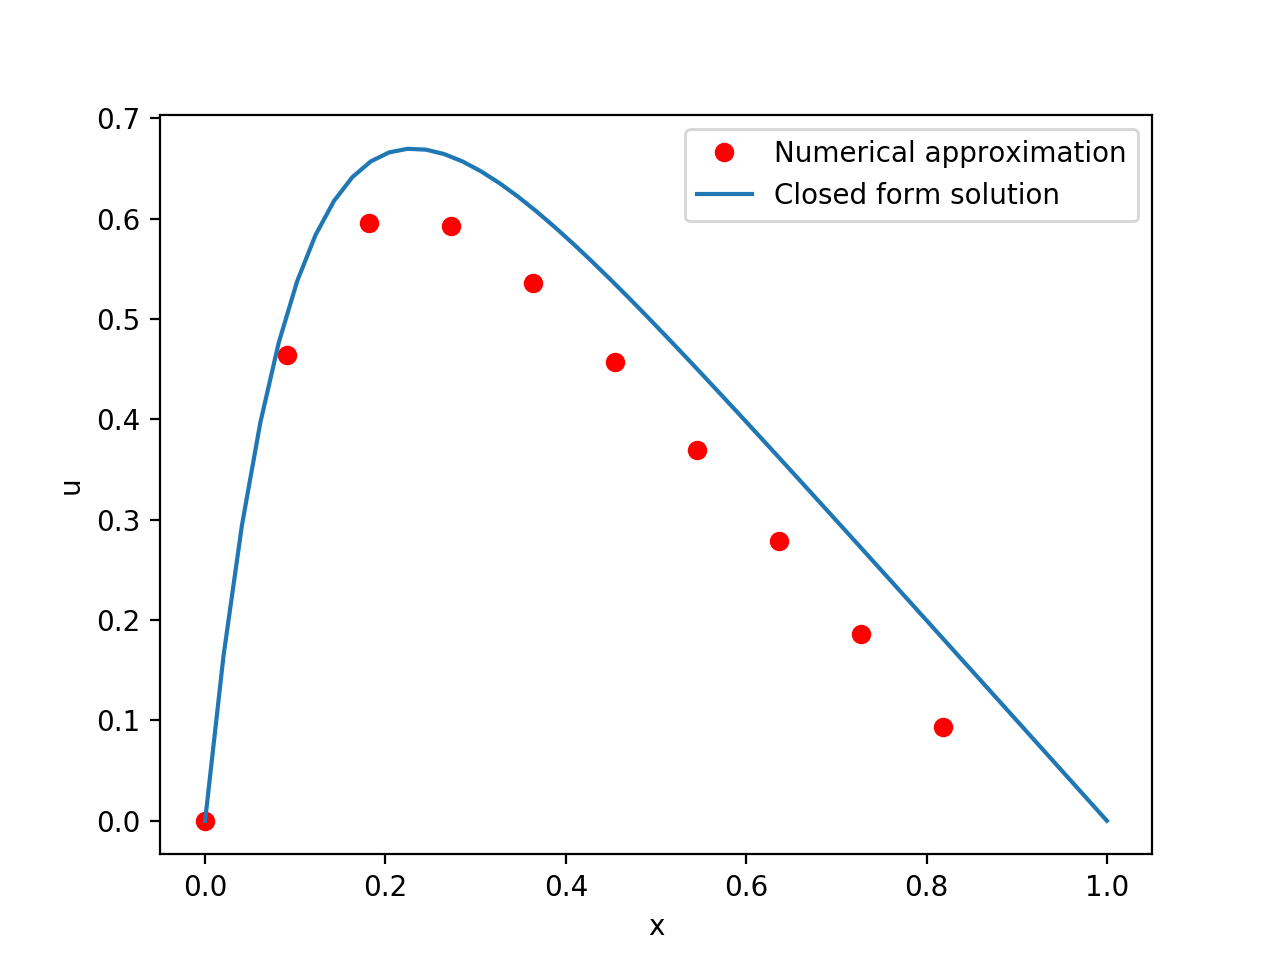
\includegraphics[width=\linewidth]{Figur/TDMA_10.png}
		\caption{TDMA for n = 10}
		\label{Fig_TDMA10}
	\end{subfigure}
	\begin{subfigure}[b]{0.3\linewidth}
		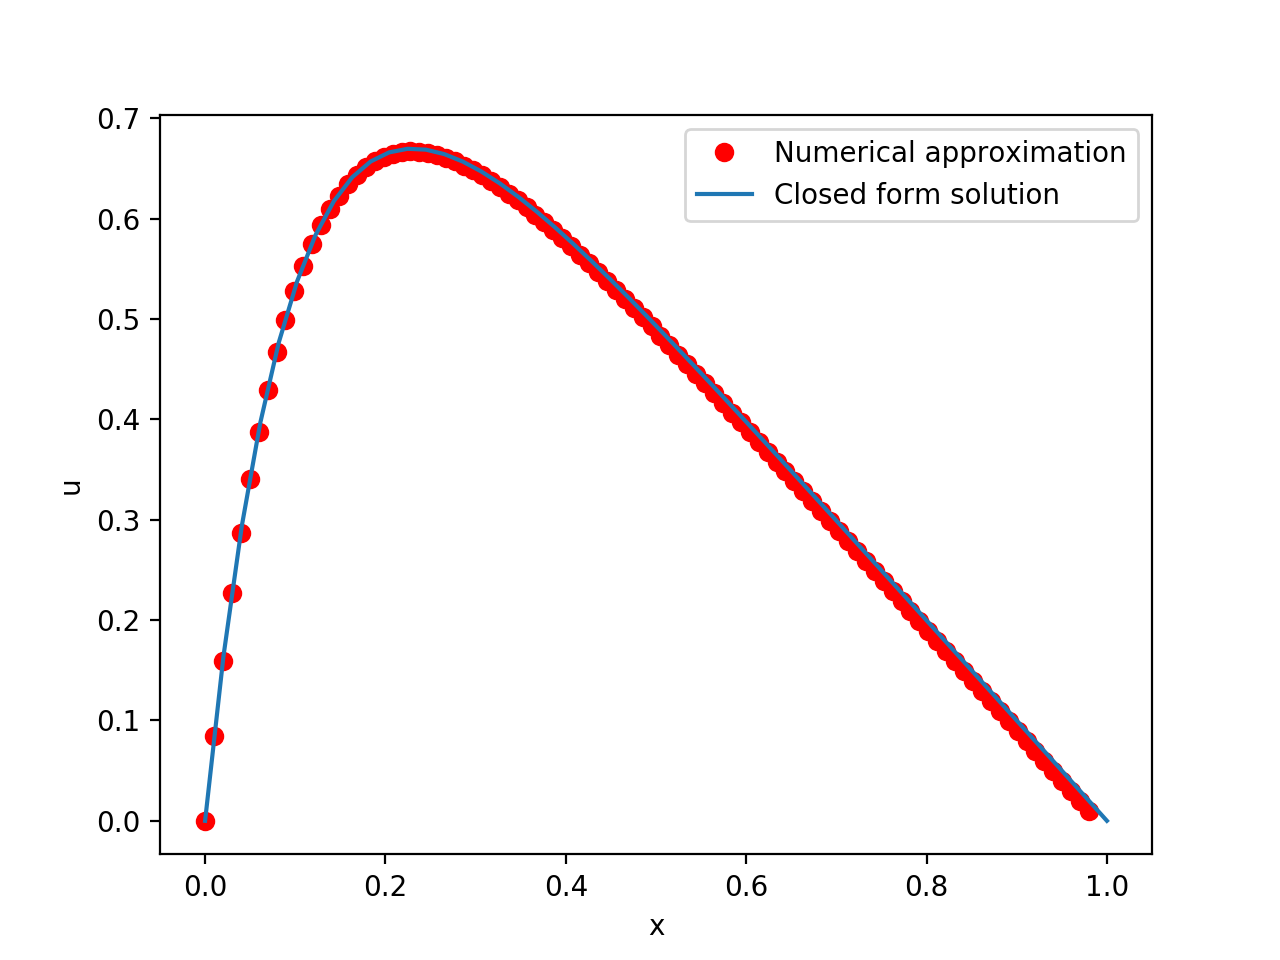
\includegraphics[width=\linewidth]{Figur/TDMA_100.png}
		\caption{TDMA for n = 100}
		\label{Fig_TDMA100}
	\end{subfigure}
	\begin{subfigure}[b]{0.3\linewidth}
		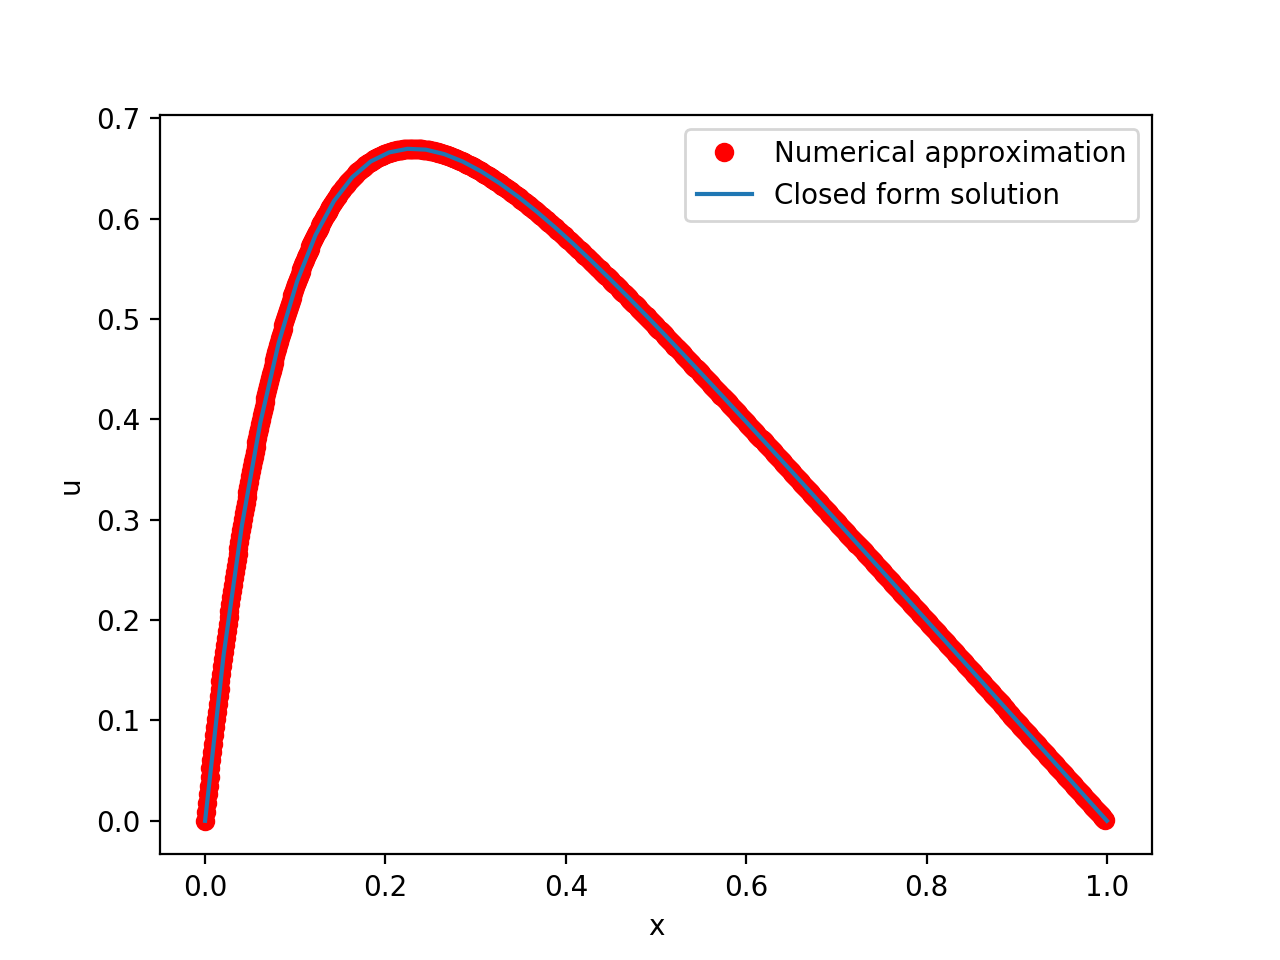
\includegraphics[width=\linewidth]{Figur/TDMA_1000.png}
		\caption{TDMA for n = 1000}
		\label{Fig_TDMA1000}
	\end{subfigure}
	\caption{Plots of the numerical - and closed form solutions for different values of $n$ devising the optimized TDMA algorithm.}
	\label{Fig_TDMA}
\end{figure}

\begin{figure}[H]
	\centering
	\begin{subfigure}[b]{0.3\linewidth}
		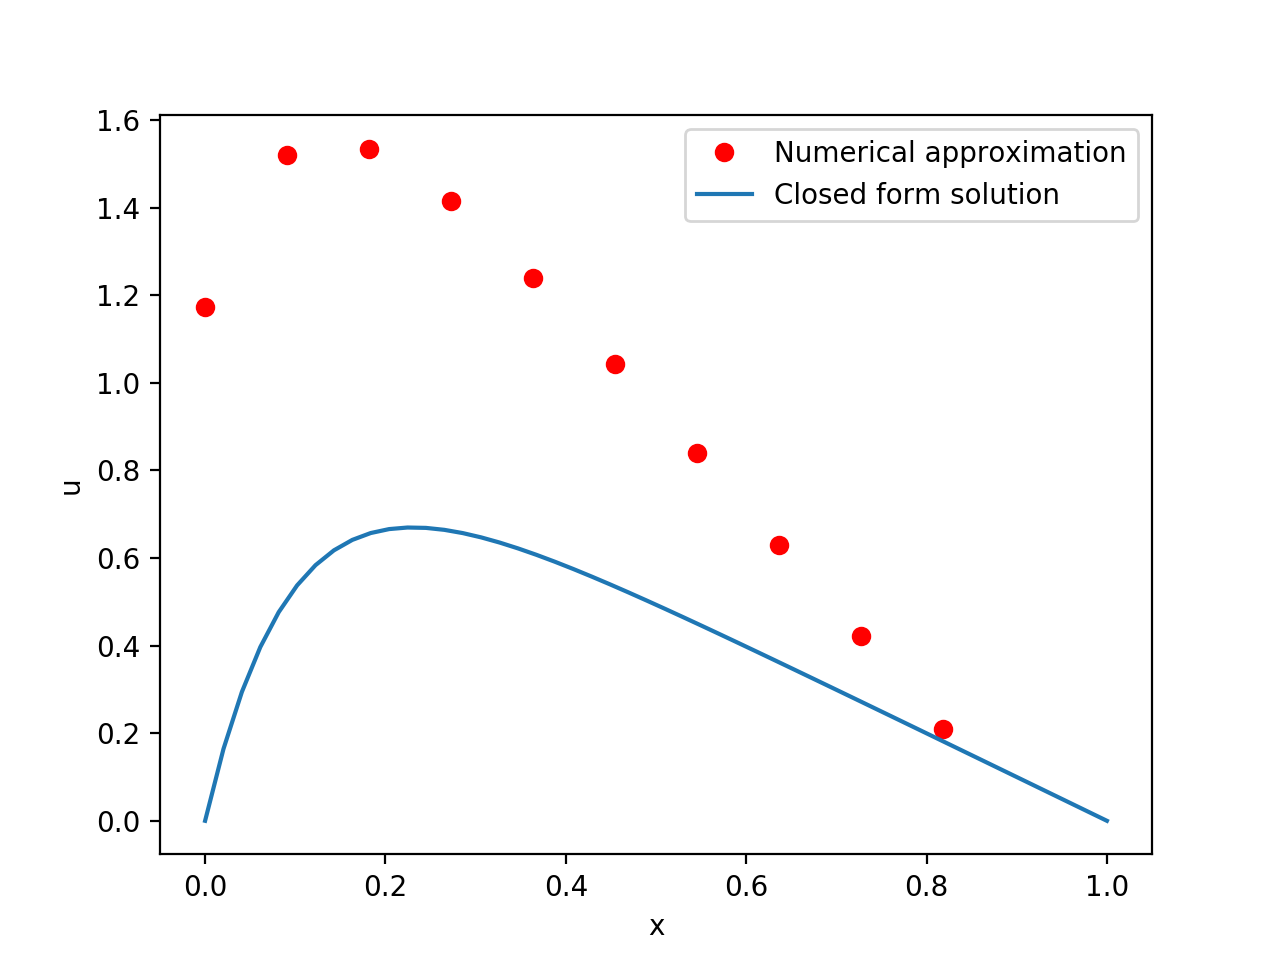
\includegraphics[width=\linewidth]{Figur/LU_10.png}
		\caption{LU for n = 10}
		\label{Fig_LU10}
	\end{subfigure}
	\begin{subfigure}[b]{0.3\linewidth}
		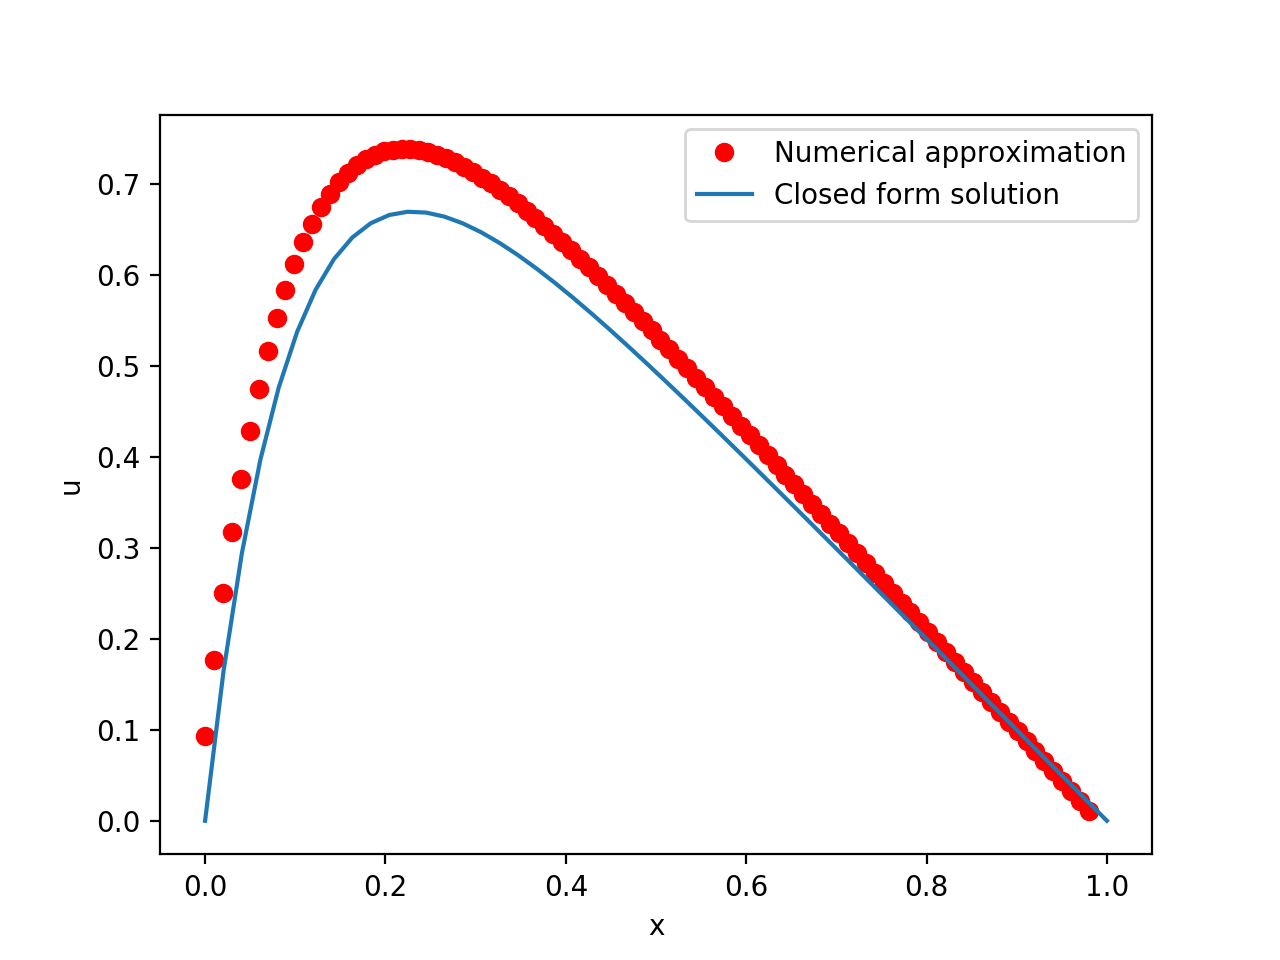
\includegraphics[width=\linewidth]{Figur/LU_100.png}
		\caption{LU for n = 100}
		\label{Fig_LU100}
	\end{subfigure}
	\begin{subfigure}[b]{0.3\linewidth}
		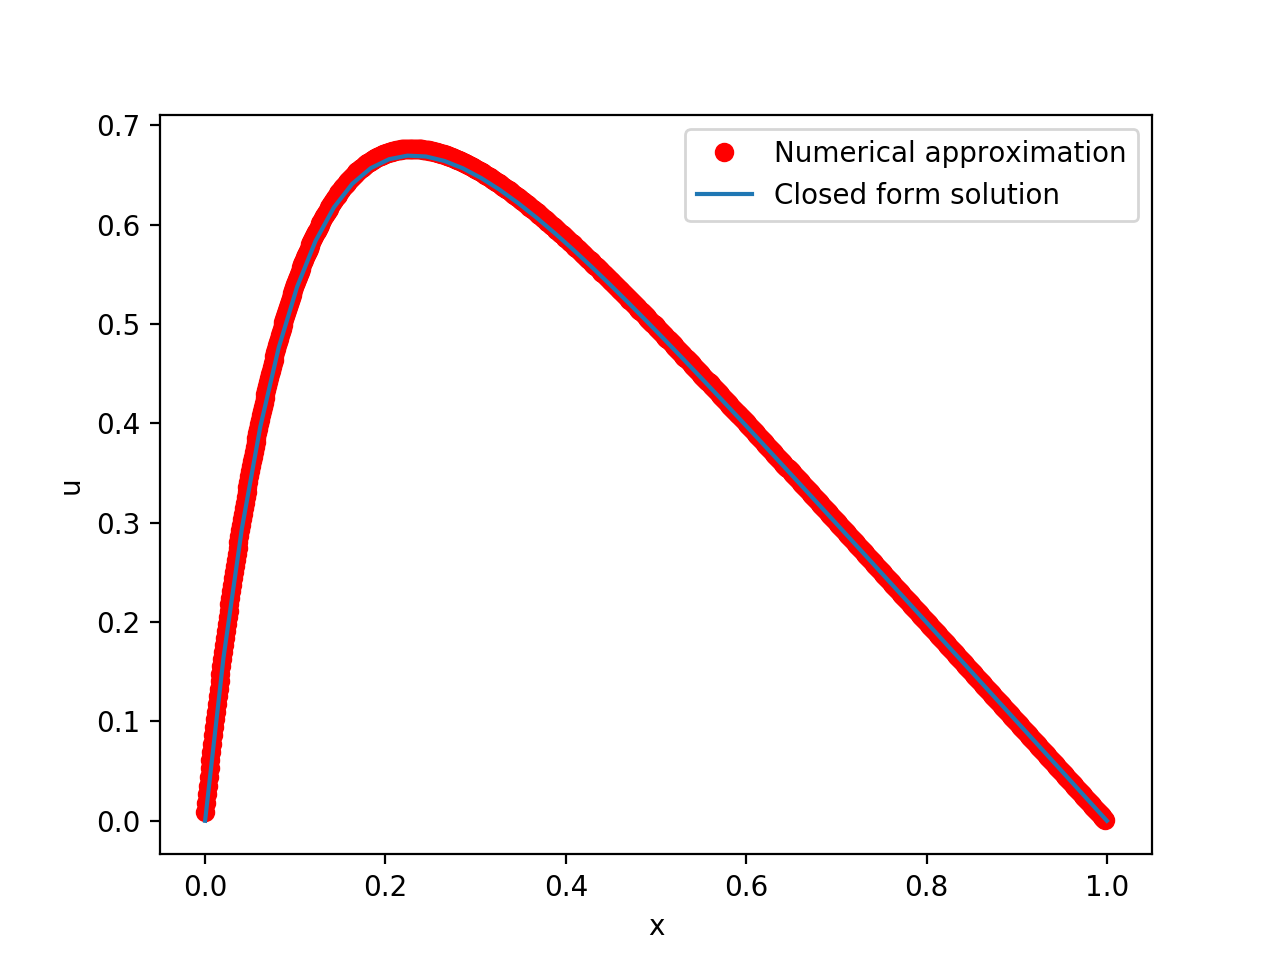
\includegraphics[width=\linewidth]{Figur/LU_1000.png}
		\caption{LU for n = 1000}
		\label{Fig_LU1000}
	\end{subfigure}
	\caption{Plots of the numerical - and closed form solutions for different values of $n$ devising the LU algorithm.}
	\label{Fig_LU}
\end{figure}

\autoref{Fig_Error} represents the associated maximum error to each step size $h$ as $n$ increases. We present this to make it clear that the numerical precision indeed increases with greater numbers of integration points. It also goes to show that there exists a minimum error for the optimized TDMA method, and it is \emph{not} associated with the smallest step size. 
\begin{figure}[H]
\centering
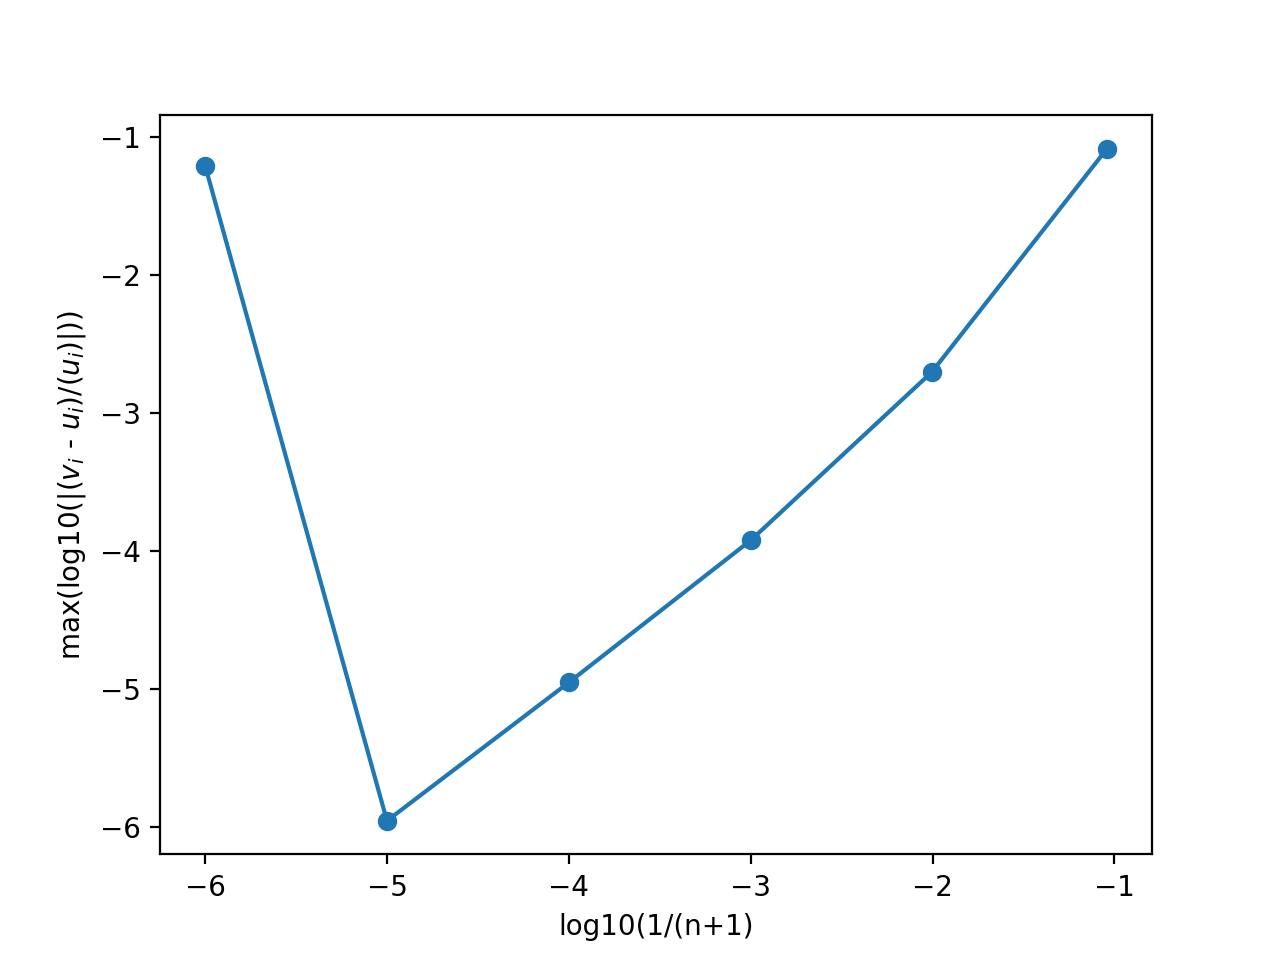
\includegraphics[width=10cm]{Figur/Error_TDMA.png}
\caption{Plot of maximum errors in the numerical solution with their associated time steps $h = 1/(n+1)$.}
\label{Fig_Error}
\end{figure}
\section{Discussion}
When prompted with a numerical problem such as the one we are studying in this project, it might be tempting to devise solvers such as Armadillo's LU - solver which has the advantage of ease of implementation. The results provided in this study, however, clearly show that when choosing a suitable solver, one must take several aspects of the solver into consideration. The main advantage of the optimized TDMA solver is that it may be tailored to the problem at hand which greatly reduces the number of FLOPs and therefore becomes a much more efficient algorithm, which is reflected in \autoref{Tab_Times}. Since the algorithm is manually implemented, it also allocates memory in a much different manner which has the advantage of solving the problem with high numerical precision whilst keeping the memory cost at a low. The results in \autoref{Tab_Times} also demonstrates this clearly; for one hundred thousand points of integration, the optimized TDMA algorithm runs about 10\% faster than the general TDMA algorithm, whilst the LU - algorithm is not even executable on a typical computer. For large $n$ where the LU - solver is executable, the general - and optimized TDMA algorithms are about one thousand times faster with the same numerical precision.\\

An important thing to take notice of, however, is that although the TDMA solver far outbests the LU solver in this case, it has its own limitations. Referring to \autoref{Fig_Error} we see that the numerical precision of the solver increases only up to a certain step size $h$, which in this case is $h = 10^{-5}$. For this step size, the maximum relative error is at its lowest, or put in other words, the numerical precision is at its highest. Increasing the points of integration to $n = 10^6$ so that $h = 10^{-6}$ dramatically lowers the numerical precision as a result of a computers ability to represent very small numbers. 
\section{Conclusion}
What we have seen so far is that there are clear advantages to devising the optimized TDMA algorithm to solve our initial problem 
$$
\begin{cases}
-u''(x) = g(x), \ x\in C^2([0,1])\\
u(0) = u(1) = 0
\end{cases}
$$
While the LU - method is more easily implemented via Armadillo, the optimized TDMA solver proves to solve the problem with great numerical precision while keeping the memory cost low. For large numbers of integration points (where the LU solver is still executable) the optimized TDMA solver is about one thousand times faster. We have also found that the TDMA solver is most precise for $n = 10^5$, a number of integration points for which the LU - solver is non-executable. More points of integration causes tremendous errors in the solution when devising the TDMA algorithm. 
\newpage
\appendix
\section{Closed form solution}
The following is a short calculation to show that the source term gives the closed form solution of Poisson's problem we have used to compare the numerical solution.
\label{Sec_CFS}
If we insert $u(x) = 1 - (1-e^{-10})x - e^{-10x}$ in \eqref{poisson} we get:
\begin{eqnarray*}
	f(x) &=& -u''(x) \\
	f(x) &=& - \left(1 - (1-e^{-10})x - e^{-10x}\right)'' = \left( -1 + x - xe^{-10} + e^{-10x} \right)'' \\
	f(x) &=& \left(1 - e^{-10} + e^{-10x}(-10) \right)' = e^{-10x}(-10)(-10) \\
	f(x) &=& 100e^{-10x}
\end{eqnarray*}

\section{Gaussian elimination of matrix}
The following are further row reductions on a general 4x4 tridiagonal matrix we used to arrive at expressions and recurrence relations for implementing the TDMA algorithm.
\label{Sec_GEM}
\begin{eqnarray*}
&
\begin{bmatrix}
b_1 & c_1 & 0 & 0 & g'_1 \\
a_1 & b_2 & c_2 & 0 & g'_2 \\
0 & a_2 & b_3 & c_3 & g'_3 \\
0 & 0 & a_3 & b_4 & g'_4
\end{bmatrix} \stackrel{\text{II} - \text{I}*a_1 / b_1}{\sim}
\begin{bmatrix}
b_1 & c_1 & 0 & 0 & g'_1\\
0 & \underbrace{b_2 - a_1 c_1 / b_1}_{\tilde{b_2}} & c_2 & 0 & \underbrace{g'_2 - g'_1 a_1 / b_1}_{\tilde{g_2}} \\
0 & a_2 & b_3 & c_3 & g'_3 \\
0 & 0 & a_3 & b_4 & g'_4
\end{bmatrix} &\\
&
\stackrel{\text{III} - \text{II}*a_2 / \tilde{b_2}}{\sim}
\begin{bmatrix}
b_1 & c_1 & 0 & 0 & g'_1\\
0 & \tilde{b}_2 & c_2 & 0 & \tilde{g}_2 \\ 
0 & 0 & \underbrace{b_3 - c_2 a_2 / \tilde{b}_2}_{\tilde{b}_3} & c_3 & \underbrace{g'_3 - \tilde{g}_2 a_2 / \tilde{b}_2}_{\tilde{g}_3} \\
0 & 0 & a_3 & b_4 & g'_4
\end{bmatrix}
\stackrel{\text{IV} - \text{III}*a_3 / \tilde{b_3}}{\sim}
\begin{bmatrix}
b_1 & c_1 & 0 & 0 & g'_1\\
0 & \tilde{b_2} & c_2 & 0 & \tilde{g}_2 \\ 
0 & 0 & \tilde{b}_3 & c_3 & \tilde{g}_3 \\
0 & 0 & 0 & \underbrace{b_4 - c_3 a_3 / \tilde{b}_3}_{\tilde{b}_4} & \underbrace{g'_4 - \tilde{g}_3 a_3 / \tilde{b}_3}_{\tilde{g}_4}
\end{bmatrix} &\\
&
= 
\begin{bmatrix}
b_1 & c_1 & 0 & 0 & g'_1\\
0 & \tilde{b_2} & c_2 & 0 & \tilde{g}_2 \\ 
0 & 0 & \tilde{b}_3 & c_3 & \tilde{g}_3 \\
0 & 0 & 0 & \tilde{b_4} & \tilde{g}_4
\end{bmatrix}&
\end{eqnarray*}


\end{document}

